\SourceLeaf{188}Die Quadrate haben daher folgende Gestalt:

\begin{center}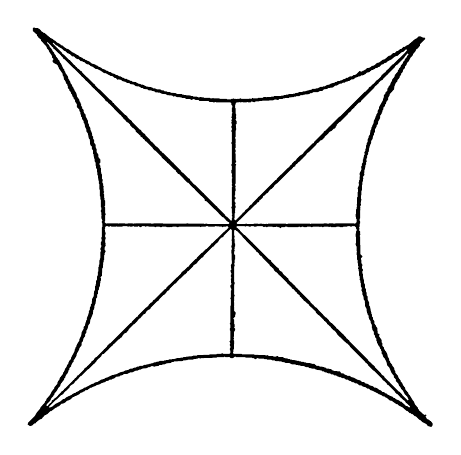
\begin{tikzpicture}[x=0.00607798cm,y=-0.00607798cm]
\fill[even odd rule] (21,10) -- (20,11) -- (20,17) -- (29,25) -- (29,27) -- (31,29) -- (31,30) -- (37,35) -- (37,37) -- (48,49) -- (50,54) -- (53,57) -- (54,60) -- (60,69) -- (60,72) -- (63,75) -- (63,77) -- (61,79) -- (61,81) -- (64,84) -- (70,87) -- (72,89) -- (75,96) -- (82,106) -- (82,109) -- (84,112) -- (85,118) -- (87,120) -- (89,124) -- (89,126) -- (92,129) -- (92,131) -- (93,132) -- (93,136) -- (96,139) -- (96,141) -- (99,144) -- (100,148) -- (102,150) -- (103,154) -- (105,156) -- (105,158) -- (108,161) -- (108,164) -- (112,170) -- (112,176) -- (117,181) -- (117,184) -- (119,186) -- (119,190) -- (121,193) -- (121,196) -- (123,198) -- (123,201) -- (126,205) -- (126,208) -- (128,211) -- (129,217) -- (132,223) -- (132,227) -- (135,231) -- (137,242) -- (139,244) -- (140,255) -- (143,258) -- (143,263) -- (146,267) -- (146,274) -- (147,275) -- (147,279) -- (148,280) -- (148,283) -- (149,284) -- (149,289) -- (151,292) -- (151,298) -- (152,299) -- (152,303) -- (154,306) -- (155,318) -- (156,319) -- (157,329) -- (158,330) -- (158,336) -- (159,337) -- (159,348) -- (160,349) -- (160,362) -- (161,363) -- (161,369) -- (162,370) -- (162,385) -- (163,386) -- (163,391) -- (162,392) -- (162,395) -- (163,396) -- (163,401) -- (164,402) -- (163,404) -- (163,408) -- (165,412) -- (165,414) -- (164,415) -- (164,418) -- (165,419) -- (165,427) -- (164,428) -- (164,448) -- (163,449) -- (164,456) -- (162,459) -- (162,464) -- (163,465) -- (163,468) -- (161,472) -- (161,474) -- (162,475) -- (162,478) -- (161,479) -- (161,492) -- (160,493) -- (160,496) -- (159,497) -- (159,505) -- (158,506) -- (158,510) -- (157,511) -- (157,520) -- (156,521) -- (156,527) -- (154,531) -- (154,537) -- (152,540) -- (152,546) -- (151,547) -- (151,550) -- (150,551) -- (150,558) -- (148,562) -- (147,572) -- (144,577) -- (143,587) -- (141,589) -- (141,592) -- (139,596) -- (139,600) -- (137,603) -- (137,607) -- (136,608) -- (136,610) -- (133,617) -- (133,621) -- (131,623) -- (131,626) -- (130,627) -- (129,633) -- (126,636) -- (126,640) -- (122,647) -- (121,654) -- (117,662) -- (117,665) -- (114,669) -- (111,675) -- (111,677) -- (109,679) -- (109,681) -- (107,684) -- (107,687) -- (100,700) -- (100,703) -- (96,707) -- (94,711) -- (94,713) -- (92,715) -- (90,720) -- (87,724) -- (87,726) -- (85,728) -- (85,730) -- (83,732) -- (83,734) -- (76,743) -- (76,745) -- (73,749) -- (71,753) -- (71,755) -- (65,762) -- (65,764) -- (60,770) -- (56,778) -- (48,787) -- (48,789) -- (46,791) -- (45,794) -- (36,804) -- (35,807) -- (28,815) -- (24,822) -- (10,836) -- (9,840) -- (14,843) -- (18,842) -- (22,838) -- (26,837) -- (27,835) -- (33,830) -- (38,828) -- (44,821) -- (50,818) -- (56,812) -- (58,812) -- (67,805) -- (70,804) -- (72,802) -- (74,802) -- (80,796) -- (83,796) -- (87,794) -- (91,790) -- (93,790) -- (99,787) -- (104,782) -- (106,782) -- (108,780) -- (110,780) -- (116,777) -- (120,773) -- (123,773) -- (125,771) -- (127,771) -- (130,768) -- (133,768) -- (140,763) -- (143,763) -- (145,761) -- (149,760) -- (154,757) -- (159,756) -- (164,753) -- (171,751) -- (173,749) -- (178,748) -- (180,746) -- (184,746) -- (187,744) -- (189,744) -- (194,740) -- (198,740) -- (199,739) -- (201,739) -- (203,737) -- (206,737) -- (211,734) -- (217,734) -- (223,731) -- (227,731) -- (235,727) -- (239,727) -- (242,725) -- (245,725) -- (248,723) -- (258,722) -- (261,720) -- (264,720) -- (267,718) -- (272,718) -- (273,719) -- (275,719) -- (276,718) -- (280,718) -- (281,717) -- (283,717) -- (285,715) -- (290,715) -- (291,714) -- (295,714) -- (299,712) -- (308,711) -- (311,709) -- (314,709) -- (315,708) -- (333,707) -- (334,706) -- (339,706) -- (340,705) -- (343,705) -- (344,704) -- (355,704) -- (356,703) -- (364,702) -- (365,701) -- (368,701) -- (370,702) -- (371,701) -- (404,700) -- (405,699) -- (419,699) -- (420,698) -- (422,698) -- (423,699) -- (428,699) -- (430,698) -- (434,701) -- (438,701) -- (442,698) -- (444,698) -- (445,699) -- (464,699) -- (465,700) -- (478,700) -- (479,701) -- (482,701) -- (484,703) -- (486,703) -- (489,701) -- (491,701) -- (492,702) -- (503,702) -- (504,703) -- (509,703) -- (510,704) -- (518,704) -- (521,706) -- (526,706) -- (527,707) -- (540,708) -- (541,709) -- (547,710) -- (548,711) -- (556,711) -- (562,714) -- (569,714) -- (570,715) -- (574,715) -- (575,716) -- (579,716) -- (580,717) -- (585,717) -- (592,720) -- (596,720) -- (599,722) -- (602,722) -- (603,723) -- (609,723) -- (612,725) -- (624,727) -- (626,729) -- (629,729) -- (631,731) -- (634,731) -- (638,733) -- (642,733) -- (644,735) -- (648,735) -- (650,737) -- (654,737) -- (656,739) -- (658,739) -- (661,741) -- (664,741) -- (667,743) -- (671,743) -- (675,746) -- (679,746) -- (681,748) -- (685,749) -- (687,751) -- (690,751) -- (695,754) -- (698,754) -- (703,758) -- (707,758) -- (709,760) -- (716,762) -- (720,765) -- (723,765) -- (726,768) -- (730,769) -- (742,775) -- (744,777) -- (746,777) -- (750,779) -- (752,781) -- (755,781) -- (757,783) -- (760,784) -- (767,790) -- (770,790) -- (780,797) -- (782,797) -- (785,800) -- (793,804) -- (801,811) -- (804,812) -- (808,816) -- (810,816) -- (812,818) -- (814,818) -- (818,822) -- (821,823) -- (827,829) -- (831,831) -- (835,835) -- (843,839) -- (846,843) -- (853,845) -- (856,841) -- (856,838) -- (852,833) -- (851,833) -- (848,830) -- (845,829) -- (843,827) -- (843,826) -- (841,824) -- (841,823) -- (843,821) -- (842,819) -- (838,820) -- (827,810) -- (827,809) -- (825,807) -- (825,805) -- (819,798) -- (816,791) -- (814,789) -- (808,779) -- (805,776) -- (805,774) -- (799,767) -- (798,763) -- (794,758) -- (792,753) -- (789,750) -- (789,748) -- (785,743) -- (783,738) -- (778,732) -- (778,729) -- (776,726) -- (776,724) -- (774,720) -- (772,718) -- (771,715) -- (767,710) -- (767,708) -- (765,706) -- (765,703) -- (762,698) -- (761,693) -- (758,687) -- (756,685) -- (754,681) -- (754,679) -- (751,676) -- (751,670) -- (749,668) -- (749,663) -- (744,656) -- (744,653) -- (745,652) -- (741,649) -- (740,638) -- (738,636) -- (737,633) -- (734,629) -- (734,624) -- (731,620) -- (731,616) -- (729,614) -- (729,610) -- (728,609) -- (728,606) -- (727,605) -- (725,594) -- (723,591) -- (723,585) -- (720,579) -- (720,572) -- (718,570) -- (718,565) -- (716,561) -- (716,556) -- (714,554) -- (714,547) -- (712,543) -- (712,537) -- (711,536) -- (711,533) -- (710,532) -- (710,525) -- (709,524) -- (709,519) -- (710,518) -- (710,516) -- (708,513) -- (708,509) -- (709,508) -- (709,506) -- (707,503) -- (707,496) -- (706,495) -- (706,492) -- (709,489) -- (709,488) -- (705,484) -- (705,465) -- (704,464) -- (704,447) -- (703,446) -- (705,442) -- (704,441) -- (704,436) -- (702,434) -- (702,432) -- (703,431) -- (702,427) -- (703,426) -- (703,420) -- (704,419) -- (704,415) -- (703,414) -- (703,410) -- (704,409) -- (704,392) -- (705,391) -- (704,389) -- (705,387) -- (704,383) -- (706,381) -- (705,376) -- (706,375) -- (706,372) -- (707,371) -- (707,369) -- (706,368) -- (706,361) -- (707,360) -- (707,351) -- (708,350) -- (708,339) -- (709,338) -- (709,332) -- (710,331) -- (710,327) -- (711,326) -- (710,322) -- (713,318) -- (713,316) -- (712,315) -- (713,313) -- (713,307) -- (714,306) -- (714,303) -- (715,302) -- (715,298) -- (717,295) -- (716,292) -- (718,290) -- (717,285) -- (719,281) -- (719,277) -- (721,274) -- (721,270) -- (723,268) -- (722,266) -- (723,264) -- (723,261) -- (724,260) -- (724,258) -- (727,251) -- (727,247) -- (730,243) -- (731,237) -- (733,234) -- (733,231) -- (735,228) -- (735,223) -- (739,216) -- (739,214) -- (741,212) -- (742,206) -- (746,199) -- (746,194) -- (749,190) -- (749,188) -- (751,186) -- (751,183) -- (753,180) -- (753,177) -- (756,174) -- (756,171) -- (758,169) -- (759,165) -- (763,160) -- (763,156) -- (766,151) -- (766,149) -- (775,139) -- (776,132) -- (779,125) -- (782,122) -- (782,120) -- (787,114) -- (787,112) -- (790,108) -- (790,106) -- (793,103) -- (794,98) -- (798,94) -- (798,91) -- (801,88) -- (802,84) -- (806,80) -- (810,72) -- (814,68) -- (815,65) -- (820,59) -- (821,56) -- (823,54) -- (824,54) -- (829,48) -- (829,45) -- (840,34) -- (840,32) -- (839,31) -- (836,31) -- (830,28) -- (827,28) -- (823,32) -- (819,34) -- (805,46) -- (800,48) -- (798,50) -- (795,50) -- (790,55) -- (788,55) -- (783,59) -- (781,59) -- (777,63) -- (774,63) -- (772,64) -- (768,68) -- (764,69) -- (756,76) -- (752,77) -- (744,83) -- (742,83) -- (738,85) -- (735,88) -- (731,90) -- (729,90) -- (727,92) -- (723,94) -- (718,95) -- (715,98) -- (714,98) -- (712,100) -- (710,100) -- (708,102) -- (703,101) -- (697,107) -- (693,109) -- (691,109) -- (687,112) -- (683,112) -- (678,115) -- (675,115) -- (673,117) -- (669,118) -- (666,120) -- (664,120) -- (661,122) -- (657,122) -- (654,124) -- (652,124) -- (651,125) -- (643,127) -- (640,129) -- (635,130) -- (630,133) -- (627,133) -- (626,134) -- (621,134) -- (615,137) -- (612,137) -- (611,138) -- (605,138) -- (602,140) -- (599,140) -- (598,141) -- (595,141) -- (594,142) -- (591,142) -- (590,143) -- (586,143) -- (582,145) -- (576,145) -- (575,146) -- (569,147) -- (568,148) -- (565,148) -- (564,149) -- (555,149) -- (554,150) -- (550,150) -- (549,151) -- (545,151) -- (544,152) -- (540,152) -- (539,153) -- (525,153) -- (524,154) -- (519,154) -- (518,155) -- (510,155) -- (509,156) -- (507,155) -- (503,155) -- (500,157) -- (491,157) -- (490,158) -- (481,158) -- (479,157) -- (477,159) -- (475,159) -- (474,158) -- (472,159) -- (456,159) -- (455,158) -- (453,158) -- (452,159) -- (447,159) -- (445,160) -- (444,159) -- (441,159) -- (439,158) -- (438,159) -- (435,159) -- (434,160) -- (426,160) -- (425,159) -- (411,159) -- (410,158) -- (398,158) -- (397,157) -- (395,158) -- (391,158) -- (390,157) -- (378,157) -- (377,156) -- (373,156) -- (372,155) -- (366,156) -- (362,154) -- (355,154) -- (354,153) -- (351,153) -- (350,152) -- (336,151) -- (335,150) -- (332,150) -- (331,149) -- (322,149) -- (318,147) -- (308,146) -- (307,145) -- (302,145) -- (299,143) -- (295,143) -- (293,141) -- (289,141) -- (286,139) -- (279,139) -- (275,137) -- (271,137) -- (269,135) -- (257,133) -- (249,129) -- (246,129) -- (245,128) -- (240,127) -- (235,124) -- (228,123) -- (226,121) -- (223,121) -- (220,119) -- (218,119) -- (216,117) -- (212,117) -- (210,115) -- (208,115) -- (203,112) -- (201,112) -- (196,109) -- (194,109) -- (189,106) -- (187,106) -- (182,103) -- (180,103) -- (175,100) -- (173,100) -- (171,98) -- (165,96) -- (163,94) -- (156,91) -- (154,89) -- (152,89) -- (150,87) -- (143,85) -- (138,81) -- (129,77) -- (127,75) -- (125,75) -- (123,73) -- (118,71) -- (115,68) -- (112,67) -- (110,65) -- (108,65) -- (106,63) -- (103,62) -- (94,55) -- (90,54) -- (88,52) -- (87,52) -- (81,47) -- (79,47) -- (76,44) -- (70,41) -- (66,37) -- (65,37) -- (60,33) -- (57,32) -- (44,21) -- (42,21) -- (40,19) -- (39,19) -- (34,13) -- (30,11) -- (25,11) -- (24,10) -- cycle
(442,433) -- (444,433) -- (446,435) -- (447,435) -- (458,446) -- (458,447) -- (466,455) -- (466,456) -- (487,477) -- (487,478) -- (489,479) -- (493,483) -- (493,484) -- (497,488) -- (498,488) -- (500,490) -- (500,491) -- (515,506) -- (515,507) -- (523,514) -- (525,518) -- (528,521) -- (529,521) -- (534,526) -- (534,527) -- (536,528) -- (552,544) -- (552,545) -- (554,547) -- (555,547) -- (557,549) -- (557,550) -- (559,551) -- (561,553) -- (561,554) -- (563,556) -- (564,556) -- (568,560) -- (568,561) -- (570,562) -- (572,564) -- (572,565) -- (578,570) -- (578,572) -- (580,573) -- (588,582) -- (589,582) -- (594,587) -- (595,587) -- (597,589) -- (597,590) -- (611,603) -- (612,606) -- (617,611) -- (618,611) -- (629,622) -- (629,623) -- (631,624) -- (635,628) -- (635,629) -- (643,636) -- (643,637) -- (649,643) -- (650,643) -- (654,647) -- (657,652) -- (676,670) -- (677,670) -- (683,676) -- (683,677) -- (715,709) -- (715,710) -- (717,711) -- (721,715) -- (721,716) -- (732,727) -- (733,727) -- (751,745) -- (751,746) -- (753,748) -- (754,748) -- (760,754) -- (760,755) -- (762,757) -- (763,757) -- (777,771) -- (777,772) -- (781,776) -- (782,776) -- (787,781) -- (788,783) -- (789,783) -- (795,789) -- (796,789) -- (799,792) -- (799,793) -- (809,802) -- (808,804) -- (806,804) -- (804,802) -- (800,801) -- (790,792) -- (788,792) -- (786,790) -- (779,787) -- (777,785) -- (774,784) -- (771,781) -- (769,781) -- (761,777) -- (759,775) -- (757,775) -- (754,772) -- (751,772) -- (748,769) -- (743,767) -- (741,765) -- (737,763) -- (734,763) -- (731,760) -- (724,758) -- (720,755) -- (715,754) -- (712,751) -- (708,751) -- (705,748) -- (698,746) -- (691,742) -- (686,741) -- (682,738) -- (678,738) -- (671,735) -- (669,733) -- (665,733) -- (662,729) -- (650,728) -- (649,727) -- (647,727) -- (643,724) -- (640,724) -- (639,723) -- (634,723) -- (632,721) -- (630,721) -- (629,720) -- (626,720) -- (625,719) -- (620,719) -- (617,717) -- (613,717) -- (608,713) -- (603,713) -- (602,712) -- (591,711) -- (590,710) -- (587,710) -- (586,709) -- (581,709) -- (580,708) -- (577,708) -- (576,707) -- (572,707) -- (571,706) -- (568,706) -- (567,705) -- (562,705) -- (561,704) -- (558,704) -- (557,703) -- (554,703) -- (553,702) -- (545,701) -- (543,699) -- (534,699) -- (532,697) -- (530,697) -- (529,698) -- (523,698) -- (522,697) -- (514,697) -- (510,695) -- (507,696) -- (506,695) -- (492,695) -- (491,694) -- (483,694) -- (482,693) -- (457,693) -- (456,692) -- (440,692) -- (438,690) -- (439,688) -- (439,683) -- (440,682) -- (440,672) -- (441,671) -- (441,665) -- (439,663) -- (440,661) -- (440,659) -- (439,658) -- (440,656) -- (440,647) -- (443,642) -- (443,640) -- (441,638) -- (441,636) -- (442,635) -- (442,631) -- (441,630) -- (441,621) -- (439,619) -- (439,618) -- (443,614) -- (443,610) -- (444,609) -- (444,606) -- (441,603) -- (441,595) -- (440,594) -- (441,592) -- (441,585) -- (440,584) -- (440,582) -- (441,581) -- (441,572) -- (442,571) -- (442,569) -- (440,567) -- (441,565) -- (441,547) -- (442,546) -- (442,543) -- (441,542) -- (441,509) -- (442,508) -- (442,506) -- (441,505) -- (441,503) -- (442,502) -- (442,495) -- (443,494) -- (443,486) -- (441,484) -- (441,478) -- (442,477) -- (441,473) -- (442,472) -- (442,468) -- (443,467) -- (443,462) -- (442,461) -- (442,452) -- (441,451) -- (441,449) -- (442,448) -- (442,446) -- (441,445) -- (441,434) -- cycle
(436,433) -- (436,453) -- (435,454) -- (436,456) -- (436,465) -- (435,466) -- (435,469) -- (436,470) -- (436,474) -- (435,475) -- (436,503) -- (434,507) -- (435,516) -- (433,518) -- (434,522) -- (435,523) -- (435,526) -- (434,527) -- (434,531) -- (435,532) -- (435,534) -- (434,535) -- (435,547) -- (433,549) -- (433,552) -- (435,556) -- (435,559) -- (434,560) -- (434,574) -- (433,575) -- (433,577) -- (434,578) -- (434,591) -- (433,592) -- (433,627) -- (432,628) -- (432,630) -- (433,631) -- (433,638) -- (432,639) -- (432,643) -- (433,644) -- (433,664) -- (431,666) -- (433,670) -- (432,672) -- (432,675) -- (433,676) -- (433,680) -- (432,681) -- (432,684) -- (433,685) -- (433,690) -- (431,692) -- (418,692) -- (417,691) -- (415,691) -- (414,692) -- (405,692) -- (404,693) -- (390,693) -- (389,694) -- (377,694) -- (376,695) -- (364,695) -- (363,696) -- (355,696) -- (354,697) -- (341,698) -- (340,699) -- (335,699) -- (334,700) -- (329,700) -- (328,701) -- (321,701) -- (320,702) -- (317,702) -- (316,703) -- (304,704) -- (303,705) -- (299,705) -- (298,706) -- (295,706) -- (294,707) -- (285,707) -- (284,708) -- (278,709) -- (277,710) -- (274,710) -- (270,712) -- (267,712) -- (266,713) -- (263,713) -- (262,714) -- (258,714) -- (257,715) -- (253,715) -- (250,717) -- (244,717) -- (241,719) -- (238,719) -- (235,721) -- (232,721) -- (228,723) -- (224,723) -- (219,726) -- (213,727) -- (210,729) -- (202,731) -- (194,735) -- (191,735) -- (190,736) -- (185,737) -- (175,742) -- (173,742) -- (168,745) -- (163,746) -- (155,751) -- (150,752) -- (146,755) -- (144,755) -- (129,763) -- (127,763) -- (125,765) -- (118,768) -- (116,770) -- (111,772) -- (109,774) -- (107,774) -- (103,776) -- (101,778) -- (90,783) -- (87,786) -- (83,787) -- (77,792) -- (67,797) -- (60,803) -- (58,803) -- (56,805) -- (54,804) -- (54,802) -- (68,788) -- (69,788) -- (78,779) -- (82,777) -- (84,775) -- (84,774) -- (96,763) -- (97,760) -- (99,758) -- (104,755) -- (107,752) -- (107,751) -- (110,748) -- (111,748) -- (120,738) -- (121,738) -- (135,724) -- (136,724) -- (147,713) -- (148,713) -- (153,707) -- (153,706) -- (163,697) -- (164,694) -- (166,692) -- (168,692) -- (175,685) -- (176,685) -- (178,683) -- (178,682) -- (184,676) -- (185,676) -- (189,671) -- (190,671) -- (199,662) -- (200,662) -- (204,658) -- (205,658) -- (208,653) -- (212,649) -- (215,648) -- (220,642) -- (220,641) -- (231,630) -- (232,630) -- (239,623) -- (239,622) -- (243,618) -- (244,618) -- (247,614) -- (249,613) -- (249,612) -- (252,609) -- (255,608) -- (257,604) -- (261,600) -- (264,599) -- (266,597) -- (266,596) -- (280,582) -- (281,582) -- (284,579) -- (284,578) -- (293,569) -- (294,569) -- (299,564) -- (299,563) -- (302,560) -- (303,560) -- (306,557) -- (306,556) -- (317,545) -- (318,545) -- (327,535) -- (328,535) -- (337,526) -- (338,526) -- (342,522) -- (342,521) -- (344,519) -- (345,519) -- (355,509) -- (355,508) -- (357,506) -- (362,503) -- (364,501) -- (364,500) -- (373,491) -- (374,491) -- (377,488) -- (377,487) -- (396,468) -- (397,468) -- (403,461) -- (404,461) -- (407,458) -- (410,453) -- (414,449) -- (417,448) -- (419,446) -- (419,445) -- (433,431) -- (434,431) -- cycle
(447,425) -- (463,425) -- (464,426) -- (466,425) -- (471,425) -- (472,426) -- (475,426) -- (476,425) -- (482,425) -- (483,426) -- (487,426) -- (488,425) -- (500,425) -- (503,427) -- (505,426) -- (507,426) -- (508,427) -- (510,427) -- (511,426) -- (521,426) -- (522,427) -- (531,426) -- (532,427) -- (535,427) -- (537,429) -- (538,429) -- (540,427) -- (546,427) -- (547,426) -- (552,426) -- (553,427) -- (575,427) -- (576,426) -- (578,426) -- (579,427) -- (581,427) -- (582,426) -- (585,426) -- (586,427) -- (592,427) -- (593,426) -- (601,426) -- (602,427) -- (604,427) -- (605,426) -- (619,426) -- (620,427) -- (622,426) -- (624,426) -- (625,427) -- (627,427) -- (628,426) -- (638,426) -- (639,427) -- (641,426) -- (643,426) -- (644,427) -- (654,427) -- (655,426) -- (661,426) -- (662,427) -- (668,427) -- (669,426) -- (677,426) -- (678,425) -- (683,425) -- (684,426) -- (686,426) -- (687,425) -- (693,425) -- (696,428) -- (696,430) -- (697,431) -- (697,435) -- (696,436) -- (696,440) -- (695,441) -- (695,447) -- (696,448) -- (696,460) -- (695,461) -- (695,464) -- (697,468) -- (697,477) -- (698,478) -- (697,480) -- (697,485) -- (698,486) -- (698,495) -- (699,496) -- (699,502) -- (700,503) -- (700,508) -- (701,509) -- (700,514) -- (701,515) -- (701,519) -- (702,520) -- (702,528) -- (703,529) -- (703,532) -- (704,533) -- (703,537) -- (705,539) -- (705,543) -- (706,544) -- (706,551) -- (708,555) -- (707,559) -- (709,563) -- (709,568) -- (711,571) -- (712,579) -- (714,581) -- (715,593) -- (718,598) -- (718,603) -- (719,604) -- (719,607) -- (720,608) -- (720,610) -- (722,612) -- (722,616) -- (723,617) -- (723,619) -- (726,623) -- (726,626) -- (729,632) -- (729,638) -- (730,639) -- (730,642) -- (733,646) -- (733,651) -- (735,653) -- (736,658) -- (738,660) -- (738,664) -- (740,667) -- (740,669) -- (743,675) -- (745,677) -- (746,681) -- (748,683) -- (748,685) -- (749,686) -- (749,691) -- (751,693) -- (753,699) -- (756,702) -- (759,708) -- (761,716) -- (765,720) -- (770,732) -- (775,738) -- (775,741) -- (779,745) -- (779,749) -- (784,754) -- (786,759) -- (788,761) -- (790,765) -- (794,769) -- (798,777) -- (803,782) -- (806,788) -- (804,790) -- (792,778) -- (792,777) -- (786,771) -- (785,771) -- (766,752) -- (766,751) -- (764,750) -- (755,741) -- (755,740) -- (752,737) -- (751,737) -- (748,734) -- (748,733) -- (735,720) -- (735,719) -- (721,706) -- (721,705) -- (682,666) -- (682,665) -- (675,659) -- (675,658) -- (669,652) -- (669,651) -- (667,650) -- (657,640) -- (656,640) -- (654,638) -- (654,637) -- (645,628) -- (644,628) -- (639,623) -- (639,622) -- (633,616) -- (632,616) -- (612,595) -- (611,595) -- (607,591) -- (606,589) -- (605,589) -- (600,584) -- (600,583) -- (577,560) -- (577,559) -- (575,558) -- (573,556) -- (573,555) -- (571,554) -- (569,552) -- (569,551) -- (555,538) -- (554,535) -- (543,525) -- (541,521) -- (537,519) -- (535,517) -- (534,514) -- (532,512) -- (531,512) -- (518,499) -- (518,497) -- (513,494) -- (480,461) -- (479,459) -- (478,459) -- (463,444) -- (462,444) -- (453,435) -- (453,434) -- (445,427) -- cycle
(429,427) -- (429,428) -- (425,433) -- (424,433) -- (395,461) -- (394,461) -- (392,463) -- (392,464) -- (383,473) -- (382,473) -- (374,481) -- (373,481) -- (363,491) -- (363,492) -- (361,494) -- (360,494) -- (347,507) -- (347,508) -- (345,510) -- (344,510) -- (336,518) -- (335,518) -- (330,523) -- (330,524) -- (299,554) -- (299,555) -- (297,557) -- (296,557) -- (287,566) -- (286,566) -- (285,568) -- (274,579) -- (273,579) -- (271,581) -- (271,582) -- (268,585) -- (267,585) -- (262,590) -- (262,591) -- (258,595) -- (257,595) -- (240,612) -- (240,613) -- (238,615) -- (237,615) -- (227,625) -- (227,626) -- (225,628) -- (224,628) -- (182,670) -- (181,670) -- (175,676) -- (175,677) -- (170,682) -- (169,682) -- (168,684) -- (153,699) -- (152,699) -- (148,703) -- (148,704) -- (145,707) -- (144,707) -- (142,709) -- (142,710) -- (135,717) -- (134,717) -- (133,719) -- (131,721) -- (130,721) -- (127,724) -- (127,725) -- (115,737) -- (114,737) -- (112,739) -- (112,740) -- (109,743) -- (108,743) -- (107,745) -- (105,747) -- (104,747) -- (103,749) -- (87,765) -- (86,765) -- (85,767) -- (82,770) -- (81,770) -- (68,784) -- (67,784) -- (62,789) -- (61,789) -- (59,791) -- (59,793) -- (57,795) -- (56,795) -- (50,802) -- (48,800) -- (49,797) -- (56,790) -- (59,784) -- (63,780) -- (63,779) -- (65,777) -- (65,775) -- (70,769) -- (73,763) -- (77,759) -- (78,755) -- (85,746) -- (85,744) -- (88,741) -- (88,739) -- (90,735) -- (92,733) -- (94,729) -- (94,727) -- (96,725) -- (96,722) -- (100,718) -- (100,716) -- (103,710) -- (105,708) -- (105,705) -- (107,703) -- (111,696) -- (112,690) -- (114,688) -- (117,682) -- (117,680) -- (122,674) -- (122,668) -- (124,666) -- (126,659) -- (129,655) -- (129,651) -- (132,647) -- (132,643) -- (134,640) -- (136,632) -- (139,628) -- (140,621) -- (145,609) -- (146,601) -- (148,598) -- (149,590) -- (151,586) -- (152,576) -- (154,574) -- (154,568) -- (156,566) -- (156,560) -- (158,557) -- (158,554) -- (160,550) -- (160,545) -- (161,544) -- (161,540) -- (162,539) -- (162,534) -- (161,532) -- (164,529) -- (165,513) -- (166,512) -- (167,501) -- (168,500) -- (168,496) -- (169,495) -- (169,486) -- (170,485) -- (170,481) -- (172,478) -- (172,477) -- (170,475) -- (170,469) -- (172,466) -- (172,464) -- (171,463) -- (172,461) -- (171,459) -- (171,453) -- (172,452) -- (172,449) -- (171,448) -- (171,443) -- (172,442) -- (172,439) -- (171,438) -- (170,431) -- (171,430) -- (171,427) -- (173,425) -- (177,425) -- (178,426) -- (180,426) -- (181,425) -- (183,425) -- (184,426) -- (193,426) -- (194,425) -- (196,426) -- (207,426) -- (208,425) -- (217,425) -- (218,426) -- (220,426) -- (221,425) -- (223,426) -- (228,426) -- (229,425) -- (231,425) -- (232,426) -- (239,426) -- (240,425) -- (242,425) -- (244,427) -- (246,427) -- (248,425) -- (254,425) -- (255,426) -- (261,425) -- (262,426) -- (274,426) -- (275,427) -- (277,427) -- (278,426) -- (285,426) -- (286,427) -- (289,427) -- (290,426) -- (299,426) -- (300,427) -- (307,427) -- (308,426) -- (310,427) -- (312,426) -- (320,426) -- (321,427) -- (324,427) -- (325,426) -- (369,426) -- (371,427) -- (372,426) -- (381,426) -- (382,425) -- (386,425) -- (387,426) -- (400,426) -- (401,425) -- (412,426) -- (414,425) -- (416,427) -- (417,427) -- (418,426) -- (424,426) -- (425,425) -- (427,425) -- cycle
(806,66) -- (803,69) -- (801,73) -- (798,76) -- (797,79) -- (794,82) -- (794,84) -- (789,90) -- (789,92) -- (786,95) -- (785,98) -- (783,100) -- (783,102) -- (777,109) -- (776,113) -- (771,119) -- (771,121) -- (768,126) -- (767,130) -- (764,133) -- (763,136) -- (761,138) -- (761,142) -- (757,146) -- (757,148) -- (754,151) -- (754,156) -- (753,157) -- (752,162) -- (744,176) -- (744,179) -- (741,184) -- (741,188) -- (738,192) -- (738,194) -- (736,197) -- (736,199) -- (733,205) -- (732,211) -- (730,214) -- (730,216) -- (728,219) -- (728,222) -- (726,225) -- (725,233) -- (722,238) -- (722,240) -- (720,244) -- (720,249) -- (718,252) -- (718,255) -- (717,256) -- (717,261) -- (715,265) -- (715,268) -- (713,271) -- (714,275) -- (712,278) -- (712,281) -- (711,282) -- (711,285) -- (710,286) -- (710,292) -- (708,295) -- (708,299) -- (706,301) -- (707,303) -- (707,307) -- (703,315) -- (704,321) -- (703,322) -- (703,329) -- (702,330) -- (702,333) -- (701,334) -- (702,339) -- (699,346) -- (700,348) -- (700,353) -- (699,354) -- (699,364) -- (698,365) -- (698,379) -- (697,380) -- (698,384) -- (697,385) -- (697,389) -- (696,390) -- (696,399) -- (695,400) -- (695,405) -- (696,406) -- (696,409) -- (697,410) -- (697,417) -- (694,420) -- (692,420) -- (691,419) -- (653,419) -- (652,420) -- (648,420) -- (647,419) -- (640,419) -- (639,420) -- (629,419) -- (628,420) -- (602,420) -- (601,421) -- (599,420) -- (553,420) -- (552,421) -- (550,421) -- (549,420) -- (512,420) -- (511,421) -- (509,421) -- (508,420) -- (506,421) -- (504,421) -- (503,420) -- (501,421) -- (499,420) -- (494,420) -- (493,421) -- (491,420) -- (482,420) -- (481,421) -- (468,421) -- (467,420) -- (465,420) -- (464,421) -- (448,421) -- (446,419) -- (446,418) -- (485,380) -- (486,380) -- (490,375) -- (492,375) -- (493,374) -- (493,372) -- (500,366) -- (501,363) -- (503,361) -- (504,361) -- (509,356) -- (510,356) -- (513,353) -- (513,352) -- (518,347) -- (519,347) -- (524,342) -- (524,341) -- (529,336) -- (530,336) -- (559,307) -- (560,307) -- (565,301) -- (568,300) -- (569,299) -- (569,297) -- (571,295) -- (572,295) -- (575,291) -- (576,291) -- (582,285) -- (583,285) -- (584,283) -- (592,275) -- (592,274) -- (595,271) -- (596,271) -- (613,254) -- (613,253) -- (615,251) -- (616,251) -- (622,245) -- (624,245) -- (630,239) -- (630,238) -- (638,231) -- (638,230) -- (640,228) -- (644,226) -- (649,221) -- (651,221) -- (653,219) -- (653,217) -- (655,215) -- (655,213) -- (661,207) -- (662,207) -- (679,190) -- (679,189) -- (681,187) -- (682,187) -- (686,183) -- (686,182) -- (692,177) -- (692,176) -- (694,174) -- (696,173) -- (696,172) -- (701,167) -- (704,166) -- (706,164) -- (706,163) -- (734,135) -- (734,134) -- (743,126) -- (743,125) -- (747,121) -- (751,119) -- (752,117) -- (760,109) -- (762,108) -- (762,107) -- (777,92) -- (777,91) -- (780,88) -- (781,88) -- (797,72) -- (797,71) -- (803,64) -- (804,64) -- cycle
(802,56) -- (802,58) -- (799,61) -- (799,62) -- (787,74) -- (786,74) -- (773,87) -- (772,87) -- (766,93) -- (766,94) -- (758,101) -- (758,102) -- (756,104) -- (755,104) -- (751,108) -- (750,108) -- (748,112) -- (741,119) -- (740,119) -- (732,128) -- (731,128) -- (725,134) -- (724,134) -- (722,136) -- (722,137) -- (715,144) -- (714,144) -- (662,196) -- (661,196) -- (640,217) -- (639,217) -- (638,219) -- (631,226) -- (630,226) -- (628,228) -- (628,229) -- (608,249) -- (608,250) -- (606,252) -- (605,252) -- (586,271) -- (586,272) -- (583,275) -- (578,278) -- (571,285) -- (571,286) -- (568,289) -- (567,289) -- (562,294) -- (562,295) -- (559,298) -- (558,298) -- (557,300) -- (530,326) -- (530,327) -- (528,329) -- (527,329) -- (492,364) -- (491,364) -- (490,366) -- (479,377) -- (479,378) -- (477,380) -- (476,380) -- (472,384) -- (472,385) -- (467,390) -- (466,390) -- (464,392) -- (464,393) -- (460,397) -- (459,397) -- (458,399) -- (444,413) -- (443,413) -- (441,411) -- (441,409) -- (442,408) -- (442,398) -- (443,397) -- (442,393) -- (443,392) -- (443,387) -- (444,386) -- (444,383) -- (443,382) -- (443,379) -- (444,377) -- (442,374) -- (442,369) -- (444,367) -- (444,366) -- (442,364) -- (442,361) -- (443,360) -- (443,352) -- (444,351) -- (444,347) -- (443,346) -- (444,341) -- (443,340) -- (443,337) -- (444,336) -- (444,298) -- (445,297) -- (445,296) -- (443,294) -- (443,293) -- (445,291) -- (445,289) -- (444,288) -- (444,274) -- (443,273) -- (443,271) -- (444,270) -- (444,266) -- (443,265) -- (443,262) -- (444,261) -- (444,253) -- (443,252) -- (444,250) -- (444,243) -- (443,242) -- (443,239) -- (444,238) -- (444,225) -- (445,224) -- (444,213) -- (446,211) -- (446,206) -- (444,203) -- (444,201) -- (445,200) -- (445,197) -- (444,196) -- (445,194) -- (445,191) -- (444,190) -- (444,179) -- (443,178) -- (443,171) -- (444,170) -- (444,168) -- (446,166) -- (450,166) -- (451,165) -- (453,166) -- (456,166) -- (457,165) -- (459,166) -- (467,166) -- (468,165) -- (470,166) -- (475,166) -- (477,164) -- (483,166) -- (486,164) -- (493,164) -- (494,163) -- (522,162) -- (526,160) -- (533,161) -- (535,159) -- (542,159) -- (543,158) -- (546,158) -- (547,157) -- (555,157) -- (556,156) -- (560,156) -- (561,155) -- (565,155) -- (566,154) -- (570,154) -- (571,153) -- (577,153) -- (580,151) -- (585,151) -- (586,150) -- (597,149) -- (600,147) -- (603,147) -- (606,145) -- (615,145) -- (621,142) -- (625,142) -- (628,139) -- (635,138) -- (638,136) -- (647,135) -- (652,131) -- (655,131) -- (662,127) -- (665,127) -- (668,125) -- (672,125) -- (674,123) -- (677,123) -- (679,121) -- (682,121) -- (686,118) -- (690,118) -- (695,114) -- (697,114) -- (701,112) -- (704,112) -- (706,110) -- (709,110) -- (715,107) -- (718,104) -- (723,103) -- (729,98) -- (731,98) -- (735,96) -- (737,94) -- (740,94) -- (742,92) -- (744,92) -- (749,87) -- (752,87) -- (755,84) -- (759,83) -- (762,80) -- (770,76) -- (776,71) -- (780,69) -- (782,69) -- (790,62) -- (795,60) -- (800,55) -- cycle
(61,43) -- (63,41) -- (69,47) -- (72,48) -- (74,50) -- (81,54) -- (85,58) -- (88,59) -- (92,63) -- (97,65) -- (102,70) -- (106,70) -- (110,74) -- (114,76) -- (116,76) -- (120,80) -- (123,80) -- (124,81) -- (128,82) -- (131,85) -- (135,87) -- (137,87) -- (142,91) -- (144,91) -- (151,96) -- (154,96) -- (162,100) -- (169,105) -- (172,105) -- (183,111) -- (186,111) -- (191,115) -- (193,115) -- (197,119) -- (199,118) -- (204,119) -- (208,122) -- (213,123) -- (216,125) -- (222,126) -- (224,128) -- (231,129) -- (235,132) -- (237,132) -- (238,133) -- (242,133) -- (247,136) -- (250,136) -- (252,138) -- (260,139) -- (262,141) -- (268,141) -- (269,142) -- (274,143) -- (276,145) -- (286,146) -- (289,148) -- (298,149) -- (301,151) -- (312,152) -- (314,154) -- (317,153) -- (321,155) -- (327,155) -- (328,156) -- (331,156) -- (332,157) -- (338,157) -- (340,159) -- (348,159) -- (352,161) -- (356,159) -- (360,161) -- (366,161) -- (368,163) -- (387,163) -- (389,165) -- (396,165) -- (397,166) -- (400,166) -- (401,165) -- (403,166) -- (433,166) -- (435,168) -- (435,171) -- (437,173) -- (437,177) -- (436,178) -- (436,186) -- (437,187) -- (437,189) -- (436,190) -- (436,196) -- (435,197) -- (435,198) -- (437,200) -- (435,204) -- (436,206) -- (435,208) -- (435,210) -- (436,211) -- (436,215) -- (435,216) -- (435,219) -- (436,220) -- (436,224) -- (435,225) -- (435,227) -- (436,228) -- (436,249) -- (435,250) -- (435,252) -- (436,253) -- (436,295) -- (435,296) -- (435,298) -- (436,299) -- (436,307) -- (435,308) -- (435,313) -- (437,317) -- (436,319) -- (436,322) -- (437,323) -- (437,325) -- (436,326) -- (436,334) -- (437,335) -- (436,337) -- (436,340) -- (437,341) -- (437,343) -- (436,344) -- (436,381) -- (437,383) -- (435,385) -- (435,387) -- (436,388) -- (436,398) -- (437,399) -- (437,401) -- (436,402) -- (436,404) -- (437,405) -- (437,407) -- (436,408) -- (436,413) -- (434,414) -- (425,405) -- (424,405) -- (422,403) -- (422,402) -- (405,385) -- (405,384) -- (403,383) -- (378,358) -- (377,356) -- (376,356) -- (358,338) -- (357,338) -- (348,328) -- (348,327) -- (346,325) -- (345,325) -- (333,313) -- (332,313) -- (330,311) -- (330,310) -- (314,294) -- (314,293) -- (312,292) -- (307,287) -- (307,286) -- (303,283) -- (302,281) -- (301,281) -- (292,272) -- (291,272) -- (289,270) -- (289,269) -- (287,268) -- (285,266) -- (285,265) -- (279,259) -- (278,259) -- (269,249) -- (268,249) -- (265,246) -- (265,245) -- (255,235) -- (255,234) -- (252,231) -- (251,231) -- (247,227) -- (247,226) -- (244,223) -- (243,223) -- (227,207) -- (227,206) -- (224,203) -- (223,203) -- (218,198) -- (218,197) -- (214,193) -- (213,193) -- (190,170) -- (189,168) -- (188,168) -- (186,166) -- (186,165) -- (182,161) -- (181,161) -- (159,139) -- (158,139) -- (150,131) -- (150,130) -- (123,104) -- (123,103) -- (121,101) -- (120,101) -- (115,96) -- (114,96) -- (112,94) -- (112,93) -- (110,92) -- (108,90) -- (108,89) -- (106,88) -- (97,78) -- (96,78) -- (84,66) -- (83,66) -- (81,64) -- (81,63) -- cycle
(49,41) -- (51,40) -- (59,48) -- (59,49) -- (63,52) -- (63,54) -- (65,55) -- (74,64) -- (75,64) -- (83,73) -- (83,74) -- (85,76) -- (86,76) -- (105,95) -- (106,95) -- (121,110) -- (121,111) -- (123,113) -- (124,113) -- (129,118) -- (129,119) -- (131,121) -- (132,121) -- (142,131) -- (142,132) -- (147,137) -- (148,137) -- (150,139) -- (150,140) -- (152,141) -- (169,158) -- (173,164) -- (175,164) -- (177,166) -- (177,167) -- (179,169) -- (180,169) -- (190,179) -- (190,180) -- (202,192) -- (203,192) -- (205,194) -- (205,195) -- (209,199) -- (209,200) -- (211,202) -- (212,202) -- (217,208) -- (219,208) -- (223,212) -- (224,215) -- (229,220) -- (230,220) -- (235,225) -- (235,227) -- (245,236) -- (245,238) -- (246,239) -- (248,239) -- (250,241) -- (250,242) -- (252,243) -- (254,245) -- (254,246) -- (256,248) -- (257,248) -- (271,262) -- (271,263) -- (275,267) -- (276,267) -- (289,280) -- (289,281) -- (300,291) -- (301,293) -- (302,293) -- (316,307) -- (317,307) -- (319,309) -- (319,310) -- (324,316) -- (326,316) -- (343,334) -- (345,334) -- (348,337) -- (348,338) -- (355,345) -- (356,345) -- (359,348) -- (359,349) -- (372,362) -- (373,362) -- (379,368) -- (379,371) -- (380,372) -- (383,373) -- (400,390) -- (401,390) -- (416,406) -- (418,406) -- (423,411) -- (423,412) -- (428,416) -- (429,416) -- (431,418) -- (431,419) -- (429,421) -- (385,421) -- (384,420) -- (381,420) -- (379,421) -- (378,420) -- (345,420) -- (344,419) -- (342,419) -- (341,420) -- (292,420) -- (291,419) -- (273,419) -- (272,420) -- (267,420) -- (266,419) -- (236,419) -- (235,420) -- (233,419) -- (231,420) -- (229,420) -- (228,419) -- (219,419) -- (218,420) -- (213,420) -- (212,419) -- (200,419) -- (198,420) -- (197,419) -- (175,419) -- (173,420) -- (170,417) -- (170,415) -- (171,414) -- (171,402) -- (172,401) -- (172,399) -- (171,398) -- (171,386) -- (170,385) -- (170,383) -- (171,382) -- (171,372) -- (169,370) -- (170,368) -- (169,366) -- (169,359) -- (168,358) -- (168,355) -- (169,353) -- (168,352) -- (168,347) -- (167,346) -- (168,342) -- (167,341) -- (167,337) -- (165,334) -- (166,328) -- (164,326) -- (164,317) -- (163,316) -- (163,313) -- (162,312) -- (162,304) -- (161,303) -- (161,299) -- (159,296) -- (159,294) -- (161,292) -- (161,286) -- (157,281) -- (157,276) -- (153,270) -- (153,264) -- (151,260) -- (151,255) -- (148,251) -- (148,245) -- (146,243) -- (146,238) -- (144,236) -- (144,233) -- (143,232) -- (143,230) -- (140,223) -- (140,220) -- (137,215) -- (137,213) -- (135,209) -- (135,205) -- (130,195) -- (130,192) -- (128,190) -- (126,186) -- (126,182) -- (123,179) -- (123,176) -- (121,174) -- (121,170) -- (119,168) -- (119,166) -- (117,164) -- (117,161) -- (112,154) -- (111,148) -- (109,144) -- (107,142) -- (107,140) -- (105,138) -- (105,136) -- (103,134) -- (101,129) -- (99,127) -- (98,123) -- (96,121) -- (96,119) -- (94,117) -- (93,112) -- (88,105) -- (88,103) -- (86,101) -- (86,98) -- (83,95) -- (79,86) -- (76,82) -- (76,80) -- (72,76) -- (72,75) -- (68,70) -- (67,67) -- (65,65) -- (64,62) -- (61,59) -- (60,56) -- (55,50) -- (54,47) -- (49,42) -- cycle;
\end{tikzpicture}
\end{center}

Ist diese Constante für \textls{uns} die halbe Erdaxe (wonach jede im Weltraume von einem Fixstern zum andern, die $90^{0}$ von einander entfernt sind, gezogene Linie eine Tangente der \textls{Erdkugel} sein würde), so ist sie in Beziehung auf die, im täglichen Leben vorkommenden, Räume unendlich gross.

\Needspace{7\baselineskip}
Die Euklidische Geometrie gilt nur unter der Voraussetzung, dass die Constante unendlich gross sei. Nur dann ist es wahr, dass die drei Winkel eines jeden Dreiecks zwei Rechten gleich seien; auch lässt sich diess, so wie man sich den Satz, dass die Constante unendlich gross sei, geben lässt, leicht beweisen.

\begin{flushright}\textsc{Schweikart.}\}\end{flushright}

\bigskip
\noindent\hrulefill
\bigskip

\Needspace{10\baselineskip}
\begin{center}
\textsc{Gauss} an \textsc{Gerling}. Marburg, 16. März 1819.
\end{center}

.\ .\ .\ .\ .\ .\ Die Notiz von Hrn. Prof. \textsc{Schweikart} hat mir ungemein viel Vergnügen gemacht, und ich bitte ihm darüber von mir recht viel Schönes zu sagen. Es ist mir fast alles aus der Seele geschrieben. Nur bloss bei dem einen Artikel der so anfängt:

Ist diese Constante für \textls{uns} die halbe Erdaxe u.\,s.\,w., muss ich drei Bemerkungen machen:

1) sehe ich die Möglichkeit nicht ein, dass eine Constante bloss für uns gelten könne, und für andere Wesen eine andere. Ich weiss auch nicht, ob Hr. \textsc{Schw.} diess so gemeint habe, nur hat er das \textls{für uns} selbst unterstrichen.

